\chapter{Lavori Correlati}
    Il mio lavoro di tesi, essendo principalmente un porting ed una rivisitazione, si basa su strumenti precedentemente sviluppati.
    Gli strumenti in questione sono descritti nel dettaglio nei seguenti sottoparagrafi.

    \section{draw.io e mxGraph}

    \begin{figure}[htbp]
        \centering
        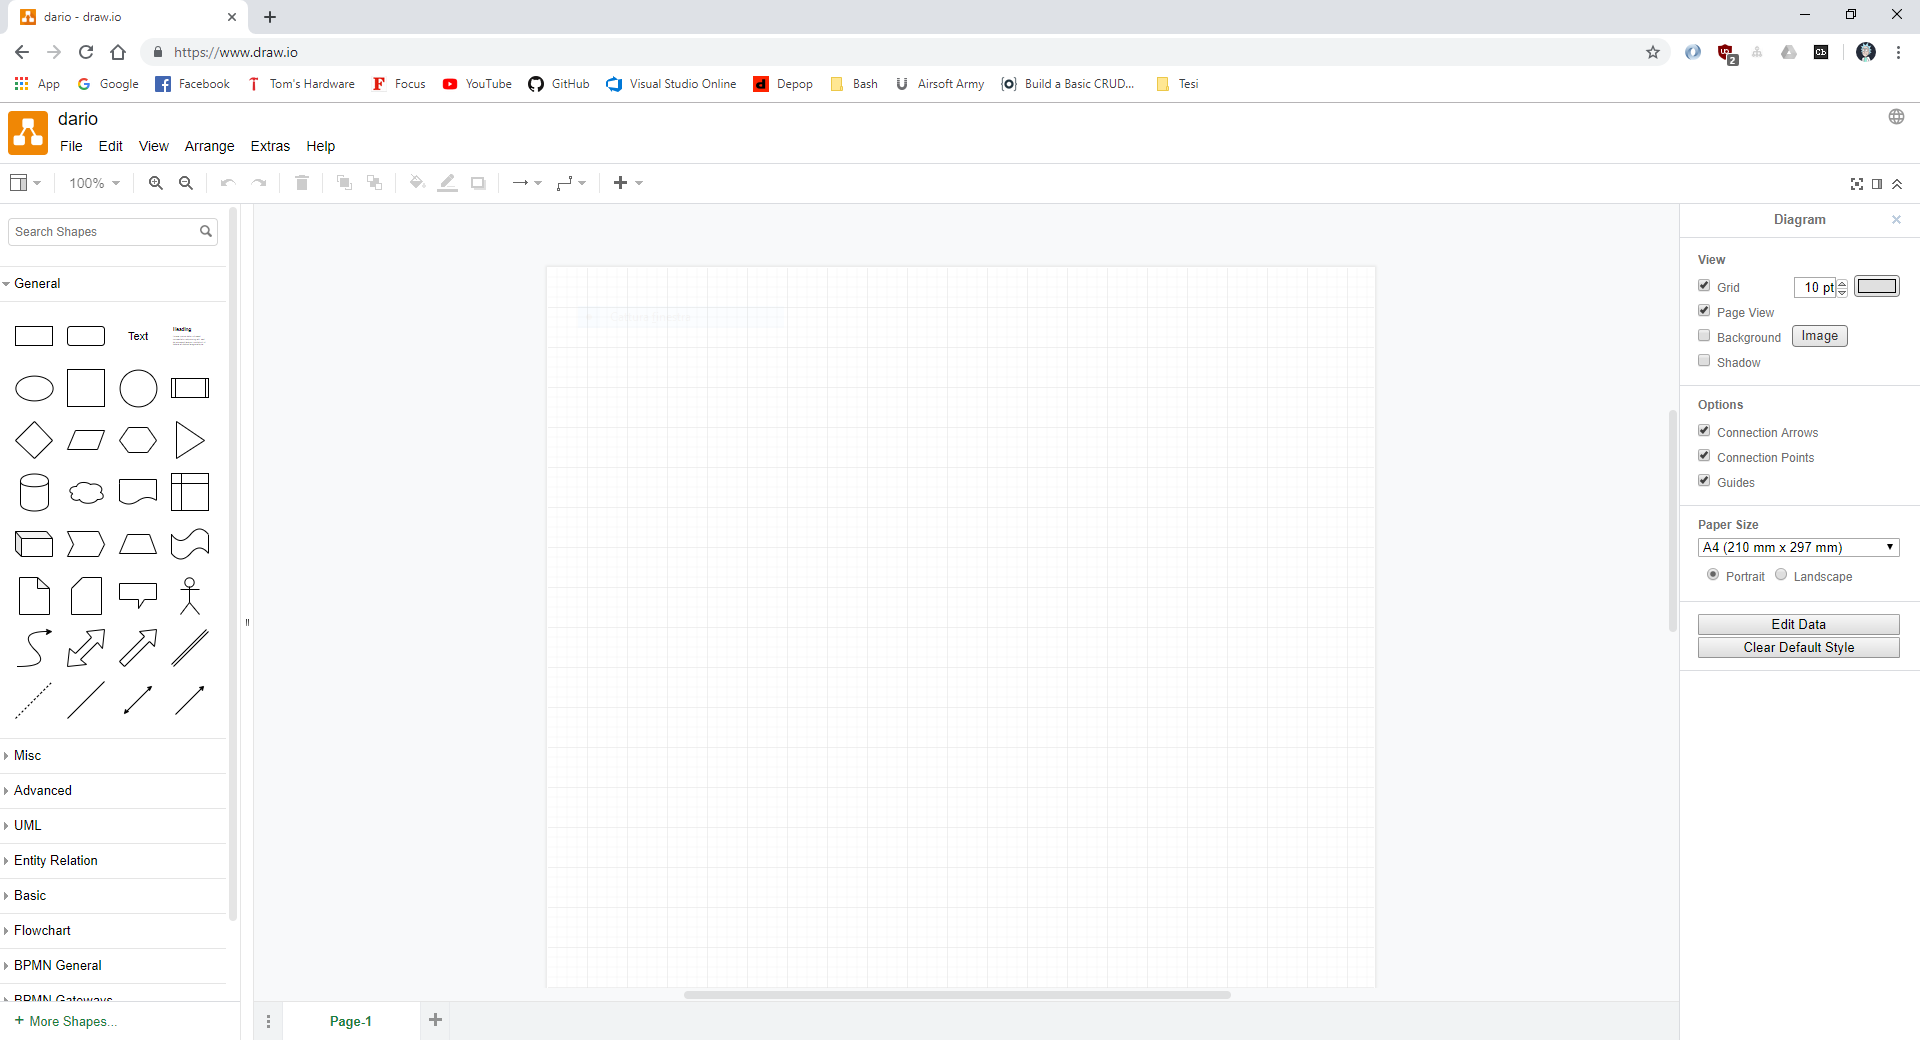
\includegraphics[scale=0.17]{Figure/drawio.png}
        \caption{Schermata di draw.io}
        \label{fig:drawio}
    \end{figure}

        TiveJS, è basato su draw.io, un'applicazione web gratis che permette agli utenti di creare diagrammi e grafi direttamente dal proprio browser web, mostrato in figura \ref{fig:drawio}. Ha un'integrazione con Google Drive e Dropbox per il salvataggio di dati che può avvenire anche con l'ausilio del localStorage del browser o attraverso il salvataggio di file sulla macchina. Draw.io è basato sulla libreria mxGraph.
        \newline
        Il software è stato sviluppato nel 2005 dalla JGraph Ltd.

    \section{LoCoMoTiVE}
        
        All'attuale stato dell'arte troviamo l'ecosistema LoCoMoTiVE, ovvero un'unione di due software, LoCoModeler e Tive. Presentato in~\cite{extending_localcontext} e~\cite{localcontext}, questo tool permette l'analisi semantica basata sul contesto locale, vista nel dettaglio nel capitolo~\ref{ch:chapter3}. Nei prossimi due paragrafi andrò ad illustrare singolarmente i due componenti di cui è composto.

        \newpage

        \subsection{LoCoModeler}
        
            \begin{figure}[htbp]
                \centering
                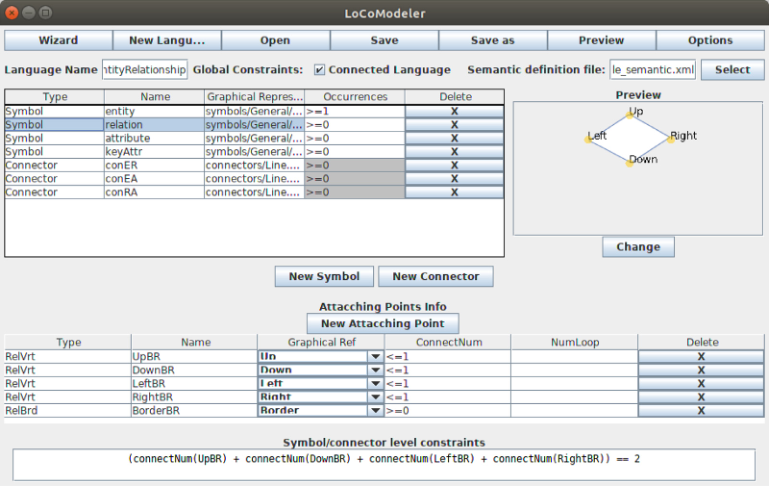
\includegraphics[scale=1.5]{Figure/locomodeler.png}
                \caption{Schermata di LoCoModeler}
                \label{fig:locomodeler}
            \end{figure}

            Come descritto in \cite{extending_localcontext}, il modulo LoCoModeler consente ai designer la creazione e la modifica del linguaggio visivo in base al contesto locale, in maniera rapida e facile. Il suo output è la definizione in formato XML del linguaggio che verrà utilizzato durante il riconoscimento dei diagrammi. Una volta che il progettista ha completato la specifica del linguaggio, può compilarlo in un ambiente web (il modulo TiVE) per consentire agli utenti di disegnare frasi e verificarne la correttezza. Durante la definizione del linguaggio, questa funzione consente al progettista di controllare la correttezza delle specifiche.
            \newline
            Una schermata principale dell'interfaccia grafica del tool è mostrata nella Figura \ref{fig:locomodeler}. Le sue componenti principali sono:
            \begin{itemize}
                \item Una casella di testo contenente il nome del linguaggio e una checkbox che sta ad indicare se il diagramma o grafo deve essere o non essere necessariamente connesso\footnote{Un grafo è detto connesso se, per ogni coppia di vertici $(u, v)\in{V}$, esiste un cammino che collega u a v.}.
                \item Una tabella riportante le informazioni principali dei simboli e dei connettori inclusi nel linguaggio. E' possibile modificare o eliminare un elemento interagendo con la riga di questo. L'utente può aggiungere nuovi simboli o connettori usando i bottoni sottostanti la tabella.
                \item Un pannello (sulla destra) mostra un'anteprima grafica del simbolo o connettore selezionato nella tabella. E' possibile cambiare la rappresentazione grafica dell'elemento utilizzando il bottone \textit{Change}.
                \item Una tabella (al centro) mostra le informazioni relative al simbolo o connettore selezionato. Ogni riga mostra un punto d'attacco e i relativi vincoli. E' possibile aggiungere nuove righe utilizzando i bottoni sovrastanti la tabella.
                \item Un'area di testo dove è possibile specificare i vincoli per il simbolo o il connettore attraverso espressioni simili al C\footnote{Linguaggio di programmazione.}.
            \end{itemize}
            La definizione di un nuovo linguaggio può avvenire grazie all'ausilio di un \textit{Wizard} diviso in tre fasi.

        \subsection{TiVE}

            \begin{figure}[htbp]
                \centering
                \includegraphics[scale=0.7]{Figure/tive.png}
                \caption{Schermata di TiVE}
                \label{fig:tive}
            \end{figure}

            Una volta definito il linguaggio, i diagrammi possono essere composti utilizzando i simboli e i connettori definiti nella sua specifica. Questo può essere fatto attraverso un editor grafico TiVE, che è un'applicazione web che consente la composizione di diagrammi direttamente dal browser web.
            \newline
            Come mostrato nella Figura~\ref{fig:tive}, l'applicazione è costituita da tre sezioni principali:
            \begin{itemize}
                \item Nella toolbar a sinistra troviamo la palette dei simboli e connettori utlizzabili per la creazione dei diagrammi.
                \item Nella zona centrale troviamo l'area di lavoro dove è possibile comporre i diagrammi trascinando gli elementi contenuti nella toolbar di sinistra.
                \item A destra troviamo la Console dove verrà mostrata la traduzione semantica o la lista di errori nel caso in cui si verificassero.
            \end{itemize}
